\documentclass[journal, letterpaper]{IEEEtran}
%\documentclass{scrartcl}

\usepackage[ngerman,english]{babel}
%\usepackage[latin1]{inputenc}
\usepackage[utf8]{inputenc}
\usepackage[T1]{fontenc}
\usepackage{amsmath}
\usepackage{amsthm}
\usepackage{amsfonts}
\usepackage{tikz}
\usepackage{verbatim}
\usepackage{subcaption}
\usepackage{algorithm}
\usepackage{algorithmic}
\usepackage[pdftex]{hyperref}

\renewcommand{\algorithmicrequire}{\textbf{Input:}}
\renewcommand{\algorithmiccomment}[1]{\ \ // #1} % C-like // Comments

\hyphenation{render}

% No clubs and widows allowed
\clubpenalty10000
\widowpenalty10000
\displaywidowpenalty=10000

\begin{document}

%\title{Simulating elastic spheres without external forces}
%\subtitle{Project 1 for class CS6491 Computer Graphics}
\title{Procedural Terrain \\
	{\large Final project for class CS6491 Computer Graphics}}
%\author{Sebastian Weiss}
\author{Sebastian Weiss \\ \today}
%\date{\today}

\maketitle

\begin{tikzpicture}[remember picture,overlay]
   \node[anchor=north east,inner sep=0pt] at (current page.north east)
              {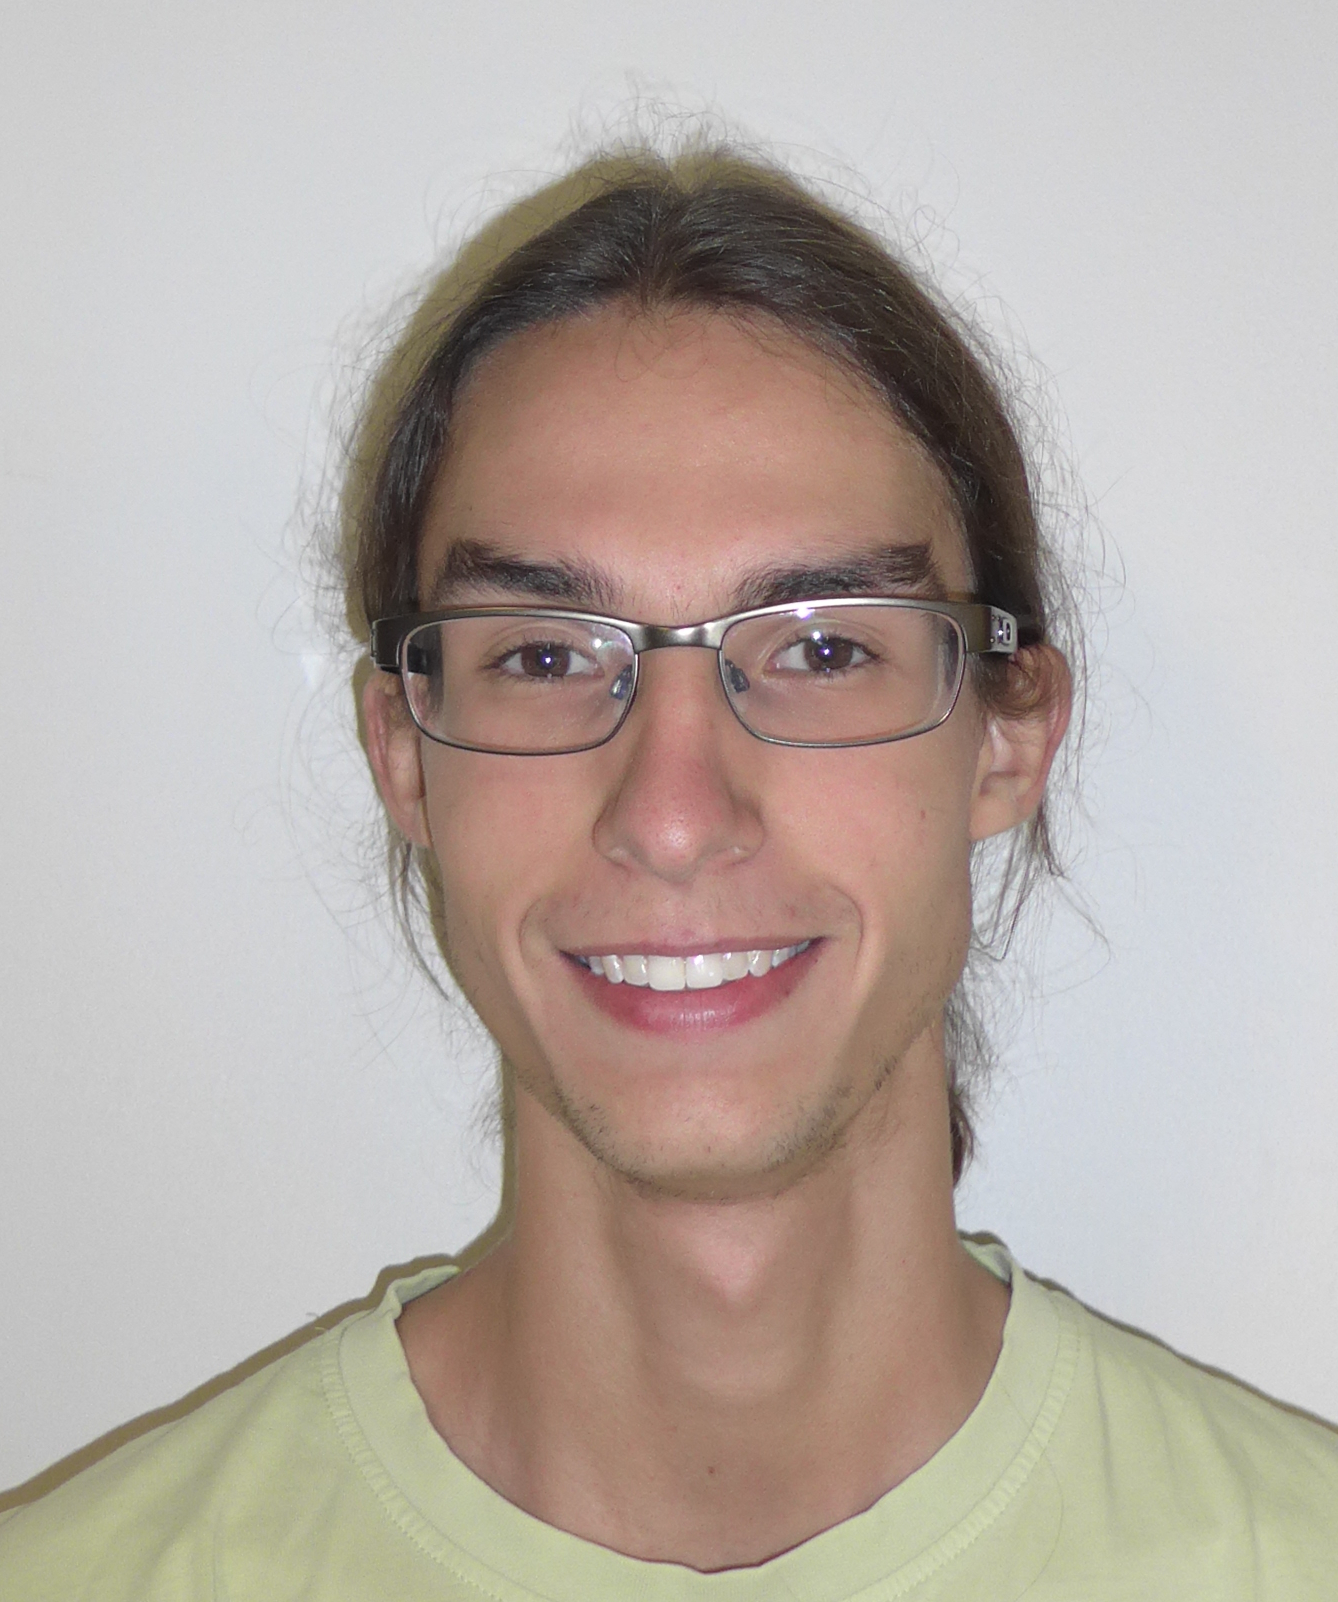
\includegraphics[scale=0.2]{pic}};
\end{tikzpicture}

\begin{abstract}
	Abstract
\end{abstract}

\section{Objective}
In this project, we want to simulate the physically correct motion of a large number of completely elastic spheres flying around in a cube.

\section{Related Work}

\section{Overview}

\section{Polygonal Map}

\subsection{Graph Datastructure}

\subsubsection{Test}

\section{Terrain Features}

\section{Hydraulic Erosion}

\section{Vegetation}

\section{Conclusion and future work}

\end{document}